\documentclass[11pt,a4paper]{article}

\usepackage[utf8]{inputenc}
\usepackage[T1]{fontenc}
\usepackage[margin=1in]{geometry}
\usepackage{amsmath,amssymb}
\usepackage{booktabs}
\usepackage{graphicx}
\usepackage{caption}
\usepackage[protrusion=true,expansion=false]{microtype}
\usepackage{array}
\usepackage{enumitem}
\usepackage{xcolor}
\usepackage[hidelinks]{hyperref}
\usepackage{url}

\providecommand{\rupee}{\textrm{Rs.}}
\newcommand{\sig}{\ensuremath{\sigma}}
\newcommand{\bsx}{\textsc{Bharat-Scam-X}}

\title{\bfseries Beyond Keywords: Attack Signatures and a Diagnostic\\
Benchmark for Multilingual Scam Detection in Indian Languages}

\author{%
  Ram Nivas Attanti\\[2pt]
  \normalsize Department of Computer Science and Business Systems\\
  \normalsize JAIN (Deemed-to-be University), Bengaluru, India\\
  \normalsize \texttt{ramnivasattanti2008@gmail.com}
}

\date{\today}

\begin{document}
\maketitle

\begin{abstract}
\noindent
Scam-message classifiers are typically evaluated on held-out samples drawn from
the same distribution as their training data, where high scores are easy to
obtain and reveal little about whether a model has learned the structure of an
attack or merely its vocabulary. We argue that the right unit of analysis is the
\emph{Attack Signature}: a typed tuple recording who the sender is impersonating,
what pretext is deployed, which asset is sought, what the recipient is asked to
do, and which persuasion levers are pulled. A signature should be invariant to
surface realisation---the same fraud written in English, Hindi, Telugu, Tamil,
Kannada, romanised transliteration or code-mixed script is one attack---and
sensitive to security semantics, so that inverting a single clause
(\emph{``share your OTP''} $\rightarrow$ \emph{``never share your OTP''})
changes it.
We formalise this notion, define four diagnostic measures over it, and release
\bsx, a constructed probe corpus of 1{,}823 labelled messages spanning nine
Indian language varieties, twelve attack families and five evaluation
conditions, including 143 minimal-edit contrast pairs whose members share
55.2\% of their tokens but carry opposite security meaning.
Evaluating four baselines, we find the gap we predicted. A character $n$-gram
classifier reaches $0.942$ macro-$F_1$ in-distribution but only $0.700$ on
semantic flips, and marks $50.7\%$ of genuine security advisories as attacks.
A structured model that predicts the signature and derives risk from it is
substantially more flip-sensitive ($0.559$ vs.\ $0.175$ flip-success) and never
fires on our hard negatives, yet it recovers the correct signature core for only
$5.6\%$ of recombined attacks that use exclusively training-seen components.
We conclude that in-distribution accuracy is close to uninformative for this
task, and release the corpus, schema and harness to make the harder questions
measurable.\footnote{Code and data: see Section~\ref{sec:availability}.}
\end{abstract}

\section{Introduction}

In calendar year 2025 the Indian Ministry of Home Affairs recorded roughly
28.15 lakh cybercrime complaints and about \mbox{\rupee\,22{,}495} crore in
reported financial losses \cite{mha2026}. A large share of this volume begins
with a text message: an SMS or messaging-app note claiming that an account is
about to be blocked, a parcel is held at customs, or a legal case has been filed,
and asking the recipient to share a one-time password, install a screen-sharing
application, or transfer money.

The natural engineering response is a classifier. The natural evaluation is a
held-out split. Both are reasonable and both, we argue, are misleading. A model
trained on messages containing \emph{OTP}, \emph{KYC}, \emph{blocked} and
\emph{urgent} can score very highly on a held-out sample containing the same
words without having represented anything about how the fraud works. Two
failure modes follow directly, and neither is visible in a standard evaluation.

First, \textbf{surface variation across languages}. India's messaging traffic is
multilingual, frequently transliterated into Latin script, and often code-mixed.
The messages \emph{``Your bank account will be blocked. Share OTP.''} and
\emph{``Mee bank account block aipothundi. OTP cheppandi.''} are the same attack.
They share almost no character $n$-grams.

Second, \textbf{security-semantic inversion}. The messages
\emph{``Your KYC has expired. Share the OTP sent to your phone.''} and
\emph{``Your KYC has expired. Never share the OTP sent to your phone with
anyone.''} differ by one clause and share most of their tokens. The first is
credential theft; the second is the advisory a bank sends to prevent it. A model
keyed on vocabulary cannot separate them, and a deployed system that flags the
second erodes exactly the trust that makes advisories work.

\paragraph{Contributions.}
\begin{enumerate}[leftmargin=1.4em,itemsep=2pt,topsep=3pt]
  \item \textbf{The Attack Signature} (Section~\ref{sec:framework}): a typed
        eight-field representation of a message's underlying attack, with an
        agreement measure \sig{} and a transparent risk map $\rho$.
  \item \textbf{The \bsx{} probe corpus} (Section~\ref{sec:corpus}): 1{,}823
        labelled messages across nine Indian language varieties and twelve
        attack families, generated by a compositional grammar so that every item
        carries a gold signature and the splits can be controlled exactly.
  \item \textbf{Four diagnostics} (Section~\ref{sec:metrics}): cross-lingual
        signature consistency, semantic-flip sensitivity, compositional
        signature recovery, and open-set behaviour.
  \item \textbf{A baseline study} (Section~\ref{sec:results}) quantifying the
        gap between in-distribution accuracy and every diagnostic, and showing
        that structured signature prediction closes part but not most of it.
\end{enumerate}

\paragraph{What this paper does not claim.}
We want to be precise about the epistemic status of our results, because it
bounds what can be concluded from them. \bsx{} is a \emph{constructed probe
corpus}, not a sample of field traffic. Its messages are composed from a
template grammar, in the tradition of SCAN \cite{lake2018scan}, COGS
\cite{kim2020cogs} and CheckList \cite{ribeiro2020checklist}. Accordingly, the
absolute numbers in Section~\ref{sec:results} are \emph{not} estimates of
deployment performance, and a model that scores well here is not thereby shown
to be deployable. What a constructed corpus buys is control: because we generate
the signature first and the surface form second, we can hold the attack fixed
while varying the language, or hold the wording nearly fixed while inverting the
security meaning. Those manipulations are what make the diagnostics possible,
and they are very hard to obtain from scraped data.

\section{Related Work}

\paragraph{SMS spam and smishing detection.}
The SMS Spam Collection \cite{almeida2011sms} established the standard
formulation---binary classification over short English messages---and remains
the most widely used benchmark. Later resources broadened coverage: SmishTank
\cite{timko2024smishtank} contributes community-reported phishing SMS, and
Salman et al.\ \cite{salman2022empirical} assemble a large scam corpus and, most
relevantly for us, show that detectors which perform well on clean text degrade
sharply under character-, word- and sentence-level perturbation. Our work
differs in the axis of stress: rather than perturbing text to preserve meaning
while breaking features, we perturb text to \emph{invert} meaning while
preserving features.

\paragraph{Multilingual and code-mixed Indic NLP.}
MuRIL \cite{khanuja2021muril} and IndicNLPSuite \cite{kakwani2020indicnlpsuite}
supply pre-trained encoders and benchmarks for Indian languages, including
transliterated text; LaBSE \cite{feng2022labse} provides language-agnostic
sentence embeddings that align translations in a shared space. These give the
representational substrate a cross-lingually invariant signature model would
need. To our knowledge no existing scam-detection benchmark evaluates whether a
detector assigns the \emph{same structured attack label} to parallel
realisations across Indian languages, which is the gap our CLSC measure targets.

\paragraph{Behavioural testing and contrast sets.}
CheckList \cite{ribeiro2020checklist} reframes NLP evaluation as behavioural
testing with targeted capability probes. Contrast sets \cite{gardner2020contrast}
perturb evaluation instances minimally so as to change the gold label, exposing
decision boundaries that held-out accuracy hides. Our semantic-flip suite is a
contrast set specialised to security semantics: the perturbation inverts the
\emph{action demanded of the recipient}, which is the field that determines
whether a message is an attack at all.

\paragraph{Compositional generalisation.}
SCAN \cite{lake2018scan} and COGS \cite{kim2020cogs} test whether models
recombine familiar primitives in unfamiliar configurations. Scam taxonomies are
naturally compositional---an actor, a pretext and a demanded action combine
fairly freely---so the same question applies directly, and is operationally
important because novel scams are typically recombinations rather than
inventions.

\paragraph{Open-set recognition.}
Closed-set classifiers assign every input to a known class. Open-set recognition
\cite{scheirer2013openset} and confidence-based out-of-distribution detection
\cite{hendrycks2017baseline} instead permit abstention. Since attackers
continually introduce new pretexts, a scam detector that cannot say ``this does
not match anything I know'' will silently mislabel novel families.

\paragraph{LLMs and the evolution of social engineering.}
Hazell \cite{hazell2023spear} documents how language models lower the cost of
personalised spear phishing, and PEEK \cite{peek2024} uses them to study how
phishing patterns evolve. If the surface form of attacks is now cheap to vary,
evaluation that rewards surface pattern-matching becomes correspondingly less
informative---which is the premise of this paper. Our tactic vocabulary draws on
Cialdini's persuasion principles \cite{cialdini2007influence}.

\section{The Attack Signature Framework}
\label{sec:framework}

\subsection{Definition}

Let $m$ be a message. Its \textbf{Attack Signature} is the tuple
\[
  S(m) \;=\; \langle a,\; p,\; t,\; i,\; c,\; g,\; T,\; E \rangle,
\]
where $a$ is the impersonated \textsc{actor}, $p$ the \textsc{pretext},
$t$ the \textsc{target} asset, $i$ the attacker \textsc{intent}, $c$ the
\textsc{action} demanded of the recipient, $g$ the kill-chain \textsc{stage},
$T \subseteq \mathcal{V}_{\text{tactic}}$ the set of persuasion
\textsc{tactics}, and $E \subseteq \mathcal{V}_{\text{evidence}}$ the set of
observable surface \textsc{evidence} cues. Each field is drawn from a closed
controlled vocabulary (Table~\ref{tab:vocab}). The six single-valued fields are
written $F_{1}$, and the two set-valued fields $F_{M}$.

We call $\kappa(m) = \langle a,p,t,i,c \rangle$ the \textbf{signature core}: the
fields that jointly determine whether, and how, a message is an attack.

\begin{table}[t]
\centering\small
\caption{Controlled vocabularies. $|\mathcal{V}|$ excludes the \texttt{none}
placeholder where present.}
\label{tab:vocab}
\begin{tabular}{@{}llp{7.4cm}@{}}
\toprule
\textbf{Field} & $|\mathcal{V}|$ & \textbf{Values (abbreviated)} \\
\midrule
\textsc{actor}    & 10 & bank, telecom, govt/police, courier, employer,
                         e-commerce, known person, utility, tech support,
                         investment platform \\
\textsc{pretext}  & 12 & account suspension, KYC expiry, parcel held, refund due,
                         job offer, prize win, legal action, bill overdue,
                         investment return, emergency help, routine notice,
                         safety advisory \\
\textsc{target}   & 7  & OTP, card PAN, UPI PIN, account credentials, funds,
                         identity document, device control \\
\textsc{intent}   & 6  & credential theft, funds transfer, malware install,
                         data harvest, advance fee, benign \\
\textsc{action}   & 9  & share code, click link, call number, install app,
                         make payment, reply, scan QR, no action, \emph{refrain} \\
\textsc{stage}    & 5  & lure, engage, extract, launder, n/a \\
\textsc{tactic}   & 7  & authority, urgency, fear, reward, social proof,
                         reciprocity, familiarity \\
\textsc{evidence} & 6  & shortened URL, phone number, monetary amount, deadline,
                         reference id, orthographic noise \\
\bottomrule
\end{tabular}
\end{table}

The \textsc{action} vocabulary includes the value \texttt{refrain}, which
encodes an instruction \emph{not} to perform an act. This single value is what
lets the framework distinguish an attack from the advisory warning against it,
and it is the mechanism the semantic-flip diagnostic probes.

\subsection{Signature agreement}

For two signatures $S, S'$ define
\[
  \sig(S,S') \;=\;
  \frac{|F_{1}| \cdot \dfrac{1}{|F_{1}|}\displaystyle\sum_{f \in F_{1}}
        \mathbb{1}[S_f = S'_f]
      \;+\; |F_{M}| \cdot \dfrac{1}{|F_{M}|}\displaystyle\sum_{f \in F_{M}}
        J(S_f, S'_f)}
       {|F_{1}| + |F_{M}|},
\]
where $J$ is Jaccard similarity and $\mathbb{1}$ the indicator. Thus
$\sig \in [0,1]$, with $\sig = 1$ iff the signatures are identical. Single-valued
fields contribute $6/8$ of the weight and set-valued fields $2/8$.

\subsection{Risk}

Risk is a deterministic function of the signature, not a separately learned
score:
\[
  \rho(S) \;=\;
  \begin{cases}
    0 & \text{if } c = \texttt{refrain} \text{ or } i = \texttt{benign},\\[3pt]
    \min\!\big(1,\; 0.9\,\lambda(i) + \beta(t)\big) & \text{otherwise,}
  \end{cases}
\]
with $\lambda$ an intent severity in $[0,1]$ and $\beta$ a small target-sensitivity
bonus (both tabulated in the released code). Deriving risk from structure rather
than fitting it directly is deliberate: it means a model can only change its risk
estimate by changing its account of \emph{what the attack is}, which is the
behaviour we want to measure.

\section{The \bsx{} Probe Corpus}
\label{sec:corpus}

\subsection{Construction}

We define twelve attack families as signature tuples instantiating documented
Indian scam modalities: bank KYC/OTP theft, account-suspension OTP theft,
KYC phishing links, ``digital arrest'' legal-threat extortion, courier-customs
payment fraud, utility disconnection callbacks, task-based job fraud,
advance-fee prize fraud, UPI refund PIN capture, remote-access tech support
fraud, investment-return fraud, and relative-in-distress fraud.

Surface realisation is compositional. For each language variety we define
independent lexical inventories for actor prefixes, pretext clauses, action
clauses (keyed by the $\langle$\textsc{action}, \textsc{target}$\rangle$ pair),
urgency intensifiers, and \emph{refrain} clauses. A message is assembled by
selecting one realisation per slot under a seeded RNG. Because the signature is
chosen first, every item carries a gold label by construction rather than by
annotation, and inter-annotator agreement is not a confound.

\paragraph{Language varieties.} Nine: English (\textsc{en}); Hindi in Devanagari
(\textsc{hi}) and romanised (\textsc{hi\_Latn}); Telugu in Telugu script
(\textsc{te}) and romanised (\textsc{te\_Latn}); Tamil (\textsc{ta}); Kannada
(\textsc{kn}); and English--Hindi (\textsc{cm\_hi}) and English--Telugu
(\textsc{cm\_te}) code-mixed varieties. Three varieties (\textsc{en},
\textsc{hi}, \textsc{hi\_Latn}) are seen in training; the remaining six are
held out entirely, so cross-lingual evaluation is zero-shot.

\subsection{Constructing minimal-edit semantic flips}

For an attack message realised as
$[\textit{prefix}] \; [\textit{pretext}] \; [\textit{action}]$, the
corresponding flip is generated with the \emph{same RNG seed}, so the prefix and
pretext clauses are string-identical, and only the action clause is replaced by
its refrain counterpart. The flip's gold signature retains the actor but sets
$p = \texttt{safety\_advisory}$, $i = \texttt{benign}$, $c = \texttt{refrain}$,
hence $\rho = 0$.

This construction is the paper's central instrument, so its minimality is
measured rather than asserted: across the 143 held-out pairs, mean token-level
Jaccard overlap is $\mathbf{0.552}$. An example pair:

\begin{quote}\small
\textbf{Attack} \; \textit{``Dear customer, Your KYC has expired. Share the OTP
sent to your phone.''} \;\; ($\rho = 1.0$)\\[2pt]
\textbf{Flip} \; \textit{``Dear customer, Your KYC has expired. Never share the
OTP sent to your phone with anyone.''} \;\; ($\rho = 0.0$)
\end{quote}

\subsection{Splits and diagnostic suites}

\begin{table}[t]
\centering\small
\caption{Corpus composition. 1{,}823 items, 1{,}563 unique strings; some items
serve more than one diagnostic. No test item is string-identical to any training
item.}
\label{tab:corpus}
\begin{tabular}{@{}llrr@{}}
\toprule
\textbf{Split} & \textbf{Suite} & \textbf{$n$} & \textbf{Purpose} \\
\midrule
train & in-distribution attacks   & 199 & seen families, seen varieties \\
train & generic benign            &  84 & class balance \\
train & hard negatives            &  13 & benign, scam vocabulary \\
train & supervised flip pairs     &  60 & makes \texttt{refrain} learnable \\
\midrule
test  & in-distribution           &  71 & held-out paraphrases \\
test  & cross-lingual             & 506 & six unseen varieties, zero-shot \\
test  & semantic flips            & 293 & 143 minimal-edit contrast pairs \\
test  & compositional             &  72 & unseen component recombinations \\
test  & open-set                  & 171 & two entirely unseen families \\
test  & parallel (CLSC)           &  90 & one signature $\times$ 9 varieties \\
test  & hard negatives            &  55 & benign, scam vocabulary \\
test  & generic benign            & 212 & ordinary traffic \\
\bottomrule
\end{tabular}
\end{table}

Table~\ref{tab:corpus} gives the composition. Three design choices deserve
comment.

\emph{Flip supervision.} Flips for five of the ten known families are placed in
\emph{training}. Without this, no model could ever predict \texttt{refrain}, and
failure on the flip suite would be a tautology rather than a finding. The
held-out flip suite therefore measures whether the attack/advisory distinction
\emph{transfers} to unseen families and varieties.

\emph{Class balance.} Training is 229 attack / 127 benign. An earlier version of
this corpus was 94\% attacks, under which every trained baseline collapsed to
predicting the majority class and scored near-perfectly on all-positive suites.
We report this because it is a trap the task invites.

\emph{Mixed evaluation conditions.} Each reported condition in
Table~\ref{tab:main} contains both attack and benign items, so macro-$F_1$ is
meaningful and a degenerate all-positive predictor cannot score well.

\section{Diagnostics}
\label{sec:metrics}

\paragraph{Cross-Lingual Signature Consistency (CLSC).}
For a parallel group $G$ containing one realisation of a single signature per
language variety, $\mathrm{CLSC}(G) = \binom{|G|}{2}^{-1}
\sum_{(u,v)} \sig(\hat S(u), \hat S(v))$, averaged over groups. This measures
\emph{self}-consistency: whether the model tells the same story about the same
attack regardless of how it is written. It is independent of whether that story
is correct, which we measure separately as agreement with gold.

\paragraph{Semantic Flip Sensitivity (SFS).}
Over contrast pairs $(m^{+}, m^{-})$ we report the \emph{flip-success rate}
$\Pr[\hat\rho(m^{+}) - \hat\rho(m^{-}) \geq 0.5]$, the mean risk drop, and the
mean token overlap of the pair. The threshold $0.5$ encodes the requirement that
a security-meaning inversion move risk across the decision midpoint, not merely
nudge it.

\paragraph{Compositional signature recovery.}
We construct four probes whose $\langle$\textsc{pretext}, \textsc{action}$\rangle$
pairings never co-occur in training although both constituents appear
separately---e.g.\ a bank KYC pretext with a call-number action. We report exact
signature-core accuracy and mean \sig{} against gold.

\paragraph{Open-set behaviour.}
Two families are withheld entirely. We score novelty by maximum softmax
probability over a family classifier \cite{hendrycks2017baseline} and report
AUROC for separating held-out-family items from known-family items.

\section{Baselines}
\label{sec:baselines}

\textbf{Keyword-Rule} flags a message when at least two of 30 hand-written
scam-indicative patterns match (covering Latin, Devanagari, Telugu, Tamil and
Kannada cues). \textbf{TFIDF-Word-LR} is word 1--2-gram TF-IDF with logistic
regression. \textbf{TFIDF-Char-LR} is character 2--5-gram TF-IDF
(\texttt{char\_wb}) with logistic regression. \textbf{Struct-Sig-Char} is our
structured model: one logistic-regression head per single-valued signature field
over the same character features, with risk computed from the predicted tuple by
$\rho$. All models see identical training data; the seed is fixed at
$20260920$.

We note explicitly that no pre-trained multilingual encoder baseline is included.
MuRIL \cite{khanuja2021muril} or LaBSE \cite{feng2022labse} are the natural
substrates for a cross-lingually invariant signature model, and we expect them
to materially improve the cross-lingual numbers in particular. Their absence is
a limitation of this study, not a claim about their performance; the released
harness is written so that adding an encoder requires replacing one feature
function.

\section{Results}
\label{sec:results}

\begin{table}[t]
\centering\small
\caption{Binary detection, macro-$F_1$. Every condition mixes attack and benign
items; condition sizes are given as $(+\text{pos}/-\text{neg})$.}
\label{tab:main}
\begin{tabular}{@{}lccccc@{}}
\toprule
& \textbf{IID} & \textbf{Cross-ling} & \textbf{Sem.\ flip} &
  \textbf{Composit.} & \textbf{Open-set} \\
& \scriptsize(+71/--33) & \scriptsize(+506/--234) & \scriptsize(+143/--150)
& \scriptsize(+72/--267) & \scriptsize(+171/--267) \\
\midrule
Keyword-Rule     & 0.706 & 0.686 & 0.570 & 0.747 & 0.640 \\
TFIDF-Word-LR    & 0.917 & \textbf{0.943} & 0.677 & 0.891 & 0.946 \\
TFIDF-Char-LR    & 0.942 & 0.936 & 0.700 & \textbf{0.920} & \textbf{0.965} \\
Struct-Sig-Char  & \textbf{1.000} & 0.888 & \textbf{0.781} & 0.918 & 0.920 \\
\bottomrule
\end{tabular}
\end{table}

\begin{table}[t]
\centering\small
\caption{False-positive rate on benign text (lower is better). ``Semantic
flips'' are genuine security advisories.}
\label{tab:fpr}
\begin{tabular}{@{}lccc@{}}
\toprule
& \textbf{Hard negatives} & \textbf{Semantic flips} & \textbf{Generic benign} \\
\midrule
Keyword-Rule     & 0.200 & 0.420 & 0.000 \\
TFIDF-Word-LR    & 0.382 & 0.560 & 0.009 \\
TFIDF-Char-LR    & 0.273 & 0.507 & 0.000 \\
Struct-Sig-Char  & \textbf{0.000} & \textbf{0.293} & 0.000 \\
\bottomrule
\end{tabular}
\end{table}

\begin{table}[t]
\centering\small
\caption{Semantic Flip Sensitivity over 143 minimal-edit contrast pairs.}
\label{tab:sfs}
\begin{tabular}{@{}lccc@{}}
\toprule
& \textbf{Flip-success} & \textbf{Mean risk drop} & \textbf{Token overlap} \\
\midrule
Keyword-Rule     & 0.028 & 0.063 & 0.552 \\
TFIDF-Word-LR    & 0.189 & 0.256 & 0.552 \\
TFIDF-Char-LR    & 0.175 & 0.277 & 0.552 \\
Struct-Sig-Char  & \textbf{0.559} & \textbf{0.494} & 0.552 \\
\bottomrule
\end{tabular}
\end{table}

\begin{figure}[t]
\centering
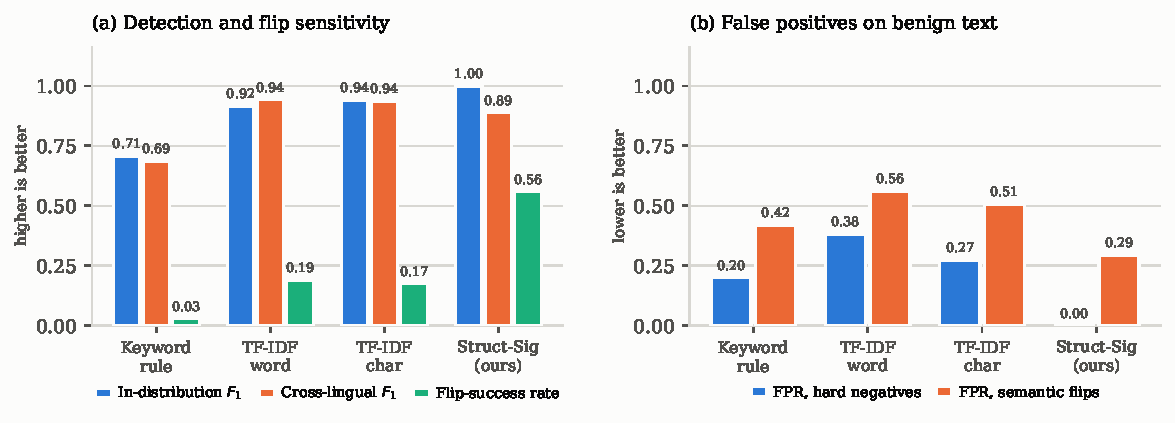
\includegraphics[width=\textwidth]{fig1_gap.pdf}
\caption{The evaluation gap. (a) In-distribution $F_1$ is high for every trained
baseline, but flip-success---the ability to recognise that inverting one clause
inverts the security meaning---is far lower. (b) All baselines fire on a
substantial fraction of genuine security advisories; the structured model fires
least.}
\label{fig:gap}
\end{figure}

\paragraph{In-distribution accuracy is close to uninformative.}
Every trained baseline exceeds $0.91$ macro-$F_1$ in-distribution
(Table~\ref{tab:main}), and the structured model is perfect. Ranking systems on
this column would put TFIDF-Char-LR and Struct-Sig-Char within $0.06$ of each
other. Their flip-success rates differ by a factor of $3.2$
(Table~\ref{tab:sfs}). The in-distribution column simply does not carry the
information a deployment decision needs.

\paragraph{Security-meaning inversion defeats lexical models.}
On pairs sharing $55.2\%$ of their tokens, TFIDF-Char-LR achieves $0.175$
flip-success, and the keyword rule $0.028$---at or below what a coin flip on the
pair would yield. Table~\ref{tab:fpr} states the operational consequence: the
word-level model flags $56.0\%$ of genuine ``never share your OTP'' advisories as
attacks. A filter with that property would suppress precisely the messages banks
send to reduce fraud.

\paragraph{Structure helps, and does not suffice.}
Struct-Sig-Char improves flip-success to $0.559$ and drives hard-negative FPR to
zero. This supports the paper's thesis: a model forced to name the demanded
action can represent the attack/advisory distinction, and this transfers to
families whose flips it never saw. But $0.559$ means it still misreads $44\%$ of
inverted messages, and it is the \emph{worst} model cross-lingually
($0.888$ vs.\ $0.943$). The reason is mechanical and worth stating plainly:
predicting six fields correctly is strictly harder than predicting one bit, so
structure converts a binary problem into six opportunities to fail. Structured
prediction is not free.

\begin{table}[t]
\centering\small
\caption{Attack Signature recovery, Struct-Sig-Char. ``Exact core'' requires all
five core fields correct.}
\label{tab:sigrec}
\begin{tabular}{@{}lcccccc@{}}
\toprule
\textbf{Suite} & $n$ & \textbf{Exact core} & \textbf{Mean \sig} &
\textbf{actor} & \textbf{intent} & \textbf{action} \\
\midrule
In-distribution & 71  & 1.000 & 0.750 & 1.000 & 1.000 & 1.000 \\
Cross-lingual   & 506 & 0.642 & 0.600 & 0.792 & 0.765 & 0.919 \\
Compositional   & 72  & 0.056 & 0.441 & 0.431 & 0.611 & 0.681 \\
Open-set        & 171 & 0.000 & 0.342 & 0.000 & 0.468 & 0.959 \\
\bottomrule
\end{tabular}
\end{table}

\paragraph{Recombination is where it breaks.}
Table~\ref{tab:sigrec} contains the study's sharpest result. On compositional
probes---built \emph{entirely} from components the model saw in training, merely
combined differently---exact signature-core recovery falls from $1.000$ to
$\mathbf{0.056}$. Per-field accuracy degrades gracefully (\textsc{action}
$0.681$, \textsc{intent} $0.611$), but the conjunction almost never survives.
Notably, binary detection on this same suite stays high ($0.918$,
Table~\ref{tab:main}): the model still says ``attack'' while being wrong about
essentially every particular of what the attack is. Since real novel scams are
overwhelmingly recombinations of familiar actors, pretexts and asks, this is the
failure mode with the most direct operational cost, and it is invisible to
binary evaluation.

\paragraph{Cross-lingual consistency degrades by script distance.}
CLSC is $1.000$ on the three training varieties and $0.787$ on the six held-out
ones ($0.837$ overall). Agreement with gold, by variety, tracks script and
lexical distance from training: \textsc{cm\_hi} $0.750$, \textsc{cm\_te} $0.738$,
\textsc{kn} $0.625$, \textsc{ta} $0.613$, \textsc{te\_Latn} $0.475$,
\textsc{te} $0.450$. Code-mixed romanised text transfers best---it shares
English tokens---while Telugu in native script transfers worst. This is the
expected behaviour of character $n$-grams and is precisely what a shared
multilingual embedding space should repair; see Section~\ref{sec:limits}.

\paragraph{Open-set numbers here are optimistic.}
Maximum-softmax-probability novelty detection reaches AUROC $0.905$. We caution
against reading this as encouraging. Our two held-out families introduce actor
and pretext vocabulary absent from training, so their novelty is lexically
visible; a genuinely hard open-set case is a new pretext expressed in familiar
vocabulary. We report the number for completeness and regard the suite as the
weakest of the five.

\section{Discussion}

Three observations generalise beyond our corpus.

\emph{The metric you optimise determines the failure you ship.} The
in-distribution column of Table~\ref{tab:main} and the flip column of
Table~\ref{tab:sfs} rank models differently. A team that reports only the former
can improve its headline number while making its product worse at the thing
users care about.

\emph{False positives on advisories are a security harm, not just an annoyance.}
Every baseline flags between $29\%$ and $56\%$ of genuine ``never share your
OTP'' messages. Anti-fraud advisories are a primary defence channel; a filter
that suppresses them degrades the defence it is meant to support. We suggest
advisory FPR be reported as standard in this literature.

\emph{Structured prediction trades breadth for depth.} Our structured model is
best where semantics matter (flips, hard negatives) and worst where surface
transfer matters (cross-lingual). This is not an argument against structure; it
is an argument for pairing structure with a representation that is already
cross-lingually aligned.

\section{Limitations}
\label{sec:limits}

\textbf{The corpus is synthetic.} Every message is template-composed. Real scam
SMS contain typos, unusual spacing, emoji, URL obfuscation, sender-ID spoofing
and length constraints we do not model, and real benign traffic is far more
diverse than ours. Our results characterise model behaviour on controlled
contrasts; they do not estimate field performance, and we would regard any
deployment claim based on them as unsupported.

\textbf{Template artifacts may be learnable.} Because attacks and benign items
are generated by different procedures, a model could in principle exploit
generation artifacts rather than meaning. We mitigate this by composing benign
messages with the same actor-prefix envelopes as attacks, and by making flip
pairs share prefix and pretext exactly; but we cannot rule it out. This is the
strongest reason to treat the corpus as diagnostic rather than as a leaderboard.

\textbf{No neural or LLM baselines.} We evaluate feature-based models only.
Pre-trained multilingual encoders and instruction-tuned LLMs will behave
differently---plausibly much better on cross-lingual transfer, and, we would
predict, still imperfectly on flips. Establishing that is the obvious next step.

\textbf{Scale and coverage.} Twelve families, nine varieties, 1{,}823 items.
Major Indian languages including Bengali, Marathi, Gujarati, Malayalam, Odia and
Punjabi are absent. Set-valued fields (\textsc{tactic}, \textsc{evidence}) are
not predicted by our structured baseline at all, which is why its mean \sig{}
is capped near $0.75$ even at perfect core accuracy.

\textbf{Single annotator of record.} Vocabularies and non-English realisations
were authored by the present author without independent linguistic review.
Native-speaker validation of the Telugu, Tamil and Kannada material is needed
before the corpus is used as a shared benchmark.

\textbf{The risk function is stipulated.} $\rho$ is hand-specified rather than
calibrated against harm data, so absolute risk values carry no external meaning;
only relative comparisons within our evaluation are interpretable.

\section{Ethical Considerations}

This work releases synthetic scam messages. We judge the marginal uplift to
attackers to be negligible: the messages are template-generated instances of
publicly documented fraud patterns, shorter and less persuasive than material
already circulating, and contain no real institution branding, no working URLs
(all links are non-resolving placeholders), no real phone numbers, and no
personal data. The defensive value of a corpus that lets researchers measure
advisory false-positive rates appears clearly greater.

We flag one asymmetric risk. A detector tuned on this corpus could be deployed
and, through the compositional and cross-lingual failures we document, silently
under-protect speakers of languages not represented in its training data. Users
of the corpus should treat Table~\ref{tab:sigrec} as a warning rather than a
scoreboard.

\section{Conclusion}

Scam detection is usually evaluated as though the problem were recognising
scam-like text. We have argued that the problem is representing an attack, and
that the two come apart measurably. A model at $0.942$ in-distribution macro-$F_1$
recovers the right attack structure for $5.6\%$ of recombined attacks and treats
half of all genuine security advisories as attacks. Making structure explicit
helps materially---tripling flip sensitivity and eliminating hard-negative false
positives---but leaves most of the gap open, and costs cross-lingual robustness.
We release the schema, the corpus and the harness so that the remaining gap can
be measured rather than assumed away.

\section*{Availability}
\label{sec:availability}

The Attack Signature schema, corpus generator, evaluation harness and all
numbers reported here are reproducible from a single fixed seed
($20260920$). The corpus is regenerated by \texttt{python3 src/generate.py} and
all tables by \texttt{python3 src/evaluate.py}.

\section*{Acknowledgements}

Portions of the software implementation and the drafting of this manuscript were
carried out with the assistance of an AI coding assistant. All design decisions,
the framework, the experimental protocol and the claims made here are the
author's, who takes full responsibility for the content.

\bibliographystyle{plain}
\bibliography{refs}

\end{document}
